\section{Materials and Methods}
% 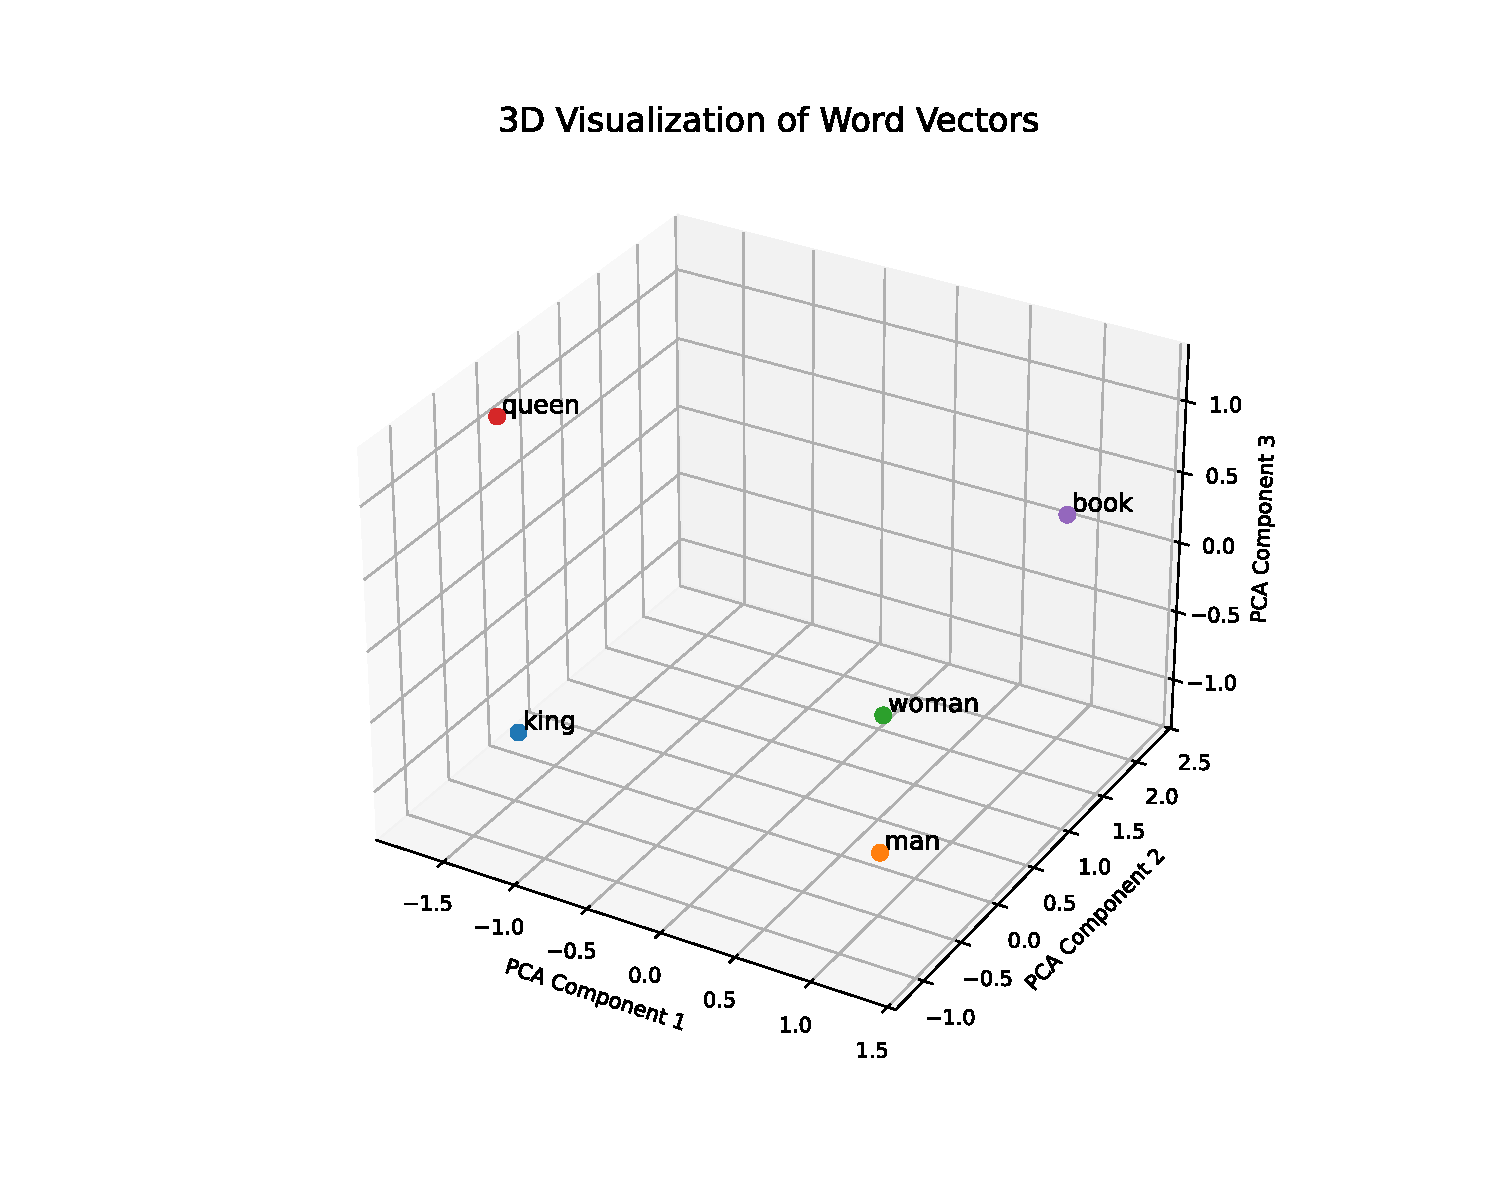
\includegraphics[trim=2cm 2cm 1cm 3cm, clip, width=\linewidth]{figures/word_vector_example.pdf}
The project used Word2Vec to transform words into high-dimensional vectors, capturing semantic relationships between words. Unlike one-hot encoding, which creates sparse vectors, Word2Vec generates dense vectors where similar words have similar representations in vector space. The model was trained with a custom dataset using Skip-Gram and Continuous Bag of Words (CBOW) techniques to learn word embeddings.

To measure the similarity between vectors, cosine similarity was employed, which calculates the cosine of the angle between vectors. Principal Component Analysis (PCA) was used to reduce the dimensionality of word vectors for a better visualization, helping to observe patterns and clusters of similar words.


\begin{figure}[H]
    \begin{minipage}{0.48\textwidth} % Left minipage takes up 48% of the text width
        \centering
        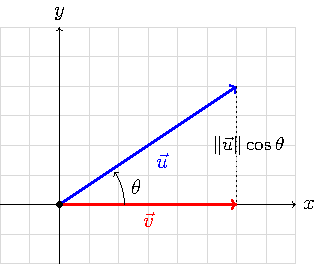
\includegraphics[width=0.6\linewidth]{figures/cosine_similarity_example.pdf}
    \end{minipage}
    \hfill
    \begin{minipage}{0.48\textwidth} % Right minipage takes up 48% of the text width
        \centering
        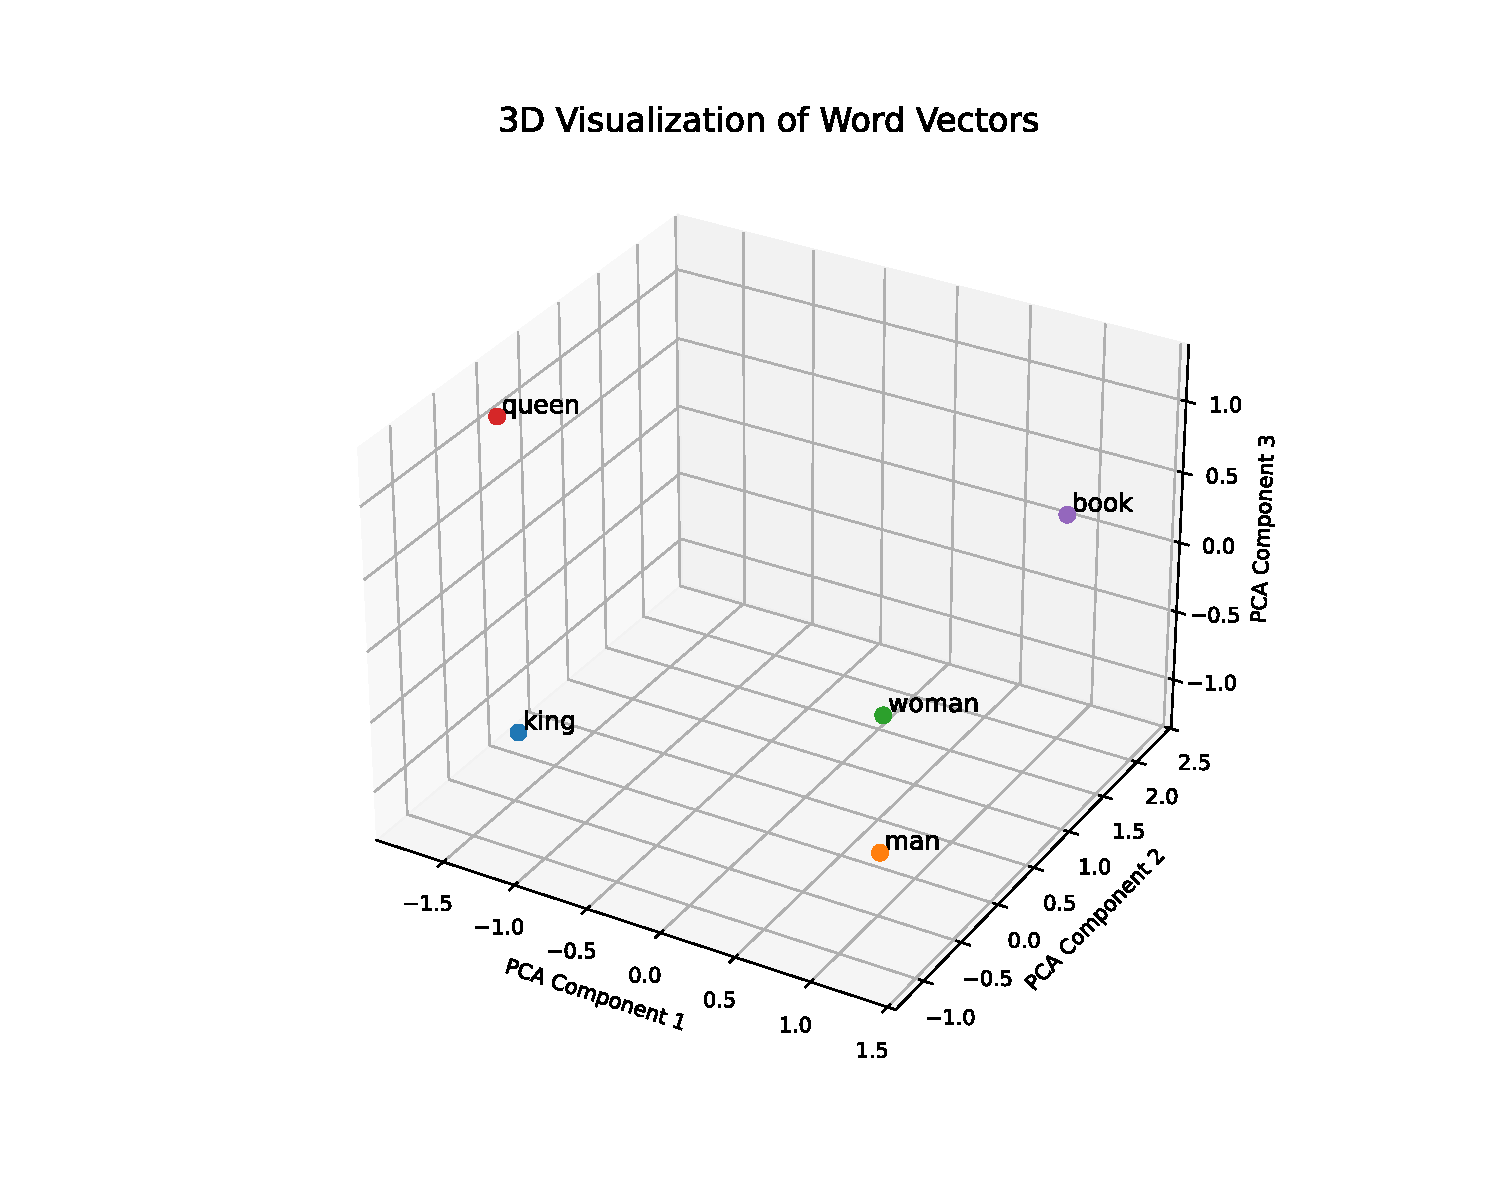
\includegraphics[trim=2cm 2cm 1cm 3cm, clip, width=\linewidth]{figures/word_vector_example.pdf}
    \end{minipage}
\end{figure}